It is now very common that an application uses multiple parallel libraries at the same time, which could be developed 
using OpenMP, TBB, Cilkplus, C++11, and other parallel libraries. 
%In Figure~\ref{fig:cholesky}, 

For example, a Cholesky Factorization~\cite{intertwine} may use OpenMP 
tasking and BLAS operations provided by Intel MKL library,
%~\footnote{The program was provided by Xavier Teruel from BSC demonstrating the interoperability problem for the INTERWinE project.}, 
which is a parallel math library. The runtime will then need to coordinate the two
parallel runtimes if the twos do not integrate, e.g. each has its own instance during the program execution. Another use case is the existence of multiple OpenMP runtime instances from either same or different libraries. These runtime instances could be created by user threads that launch into
OpenMP operations. 
%\begin{figure}[h!]
%  \centering
%      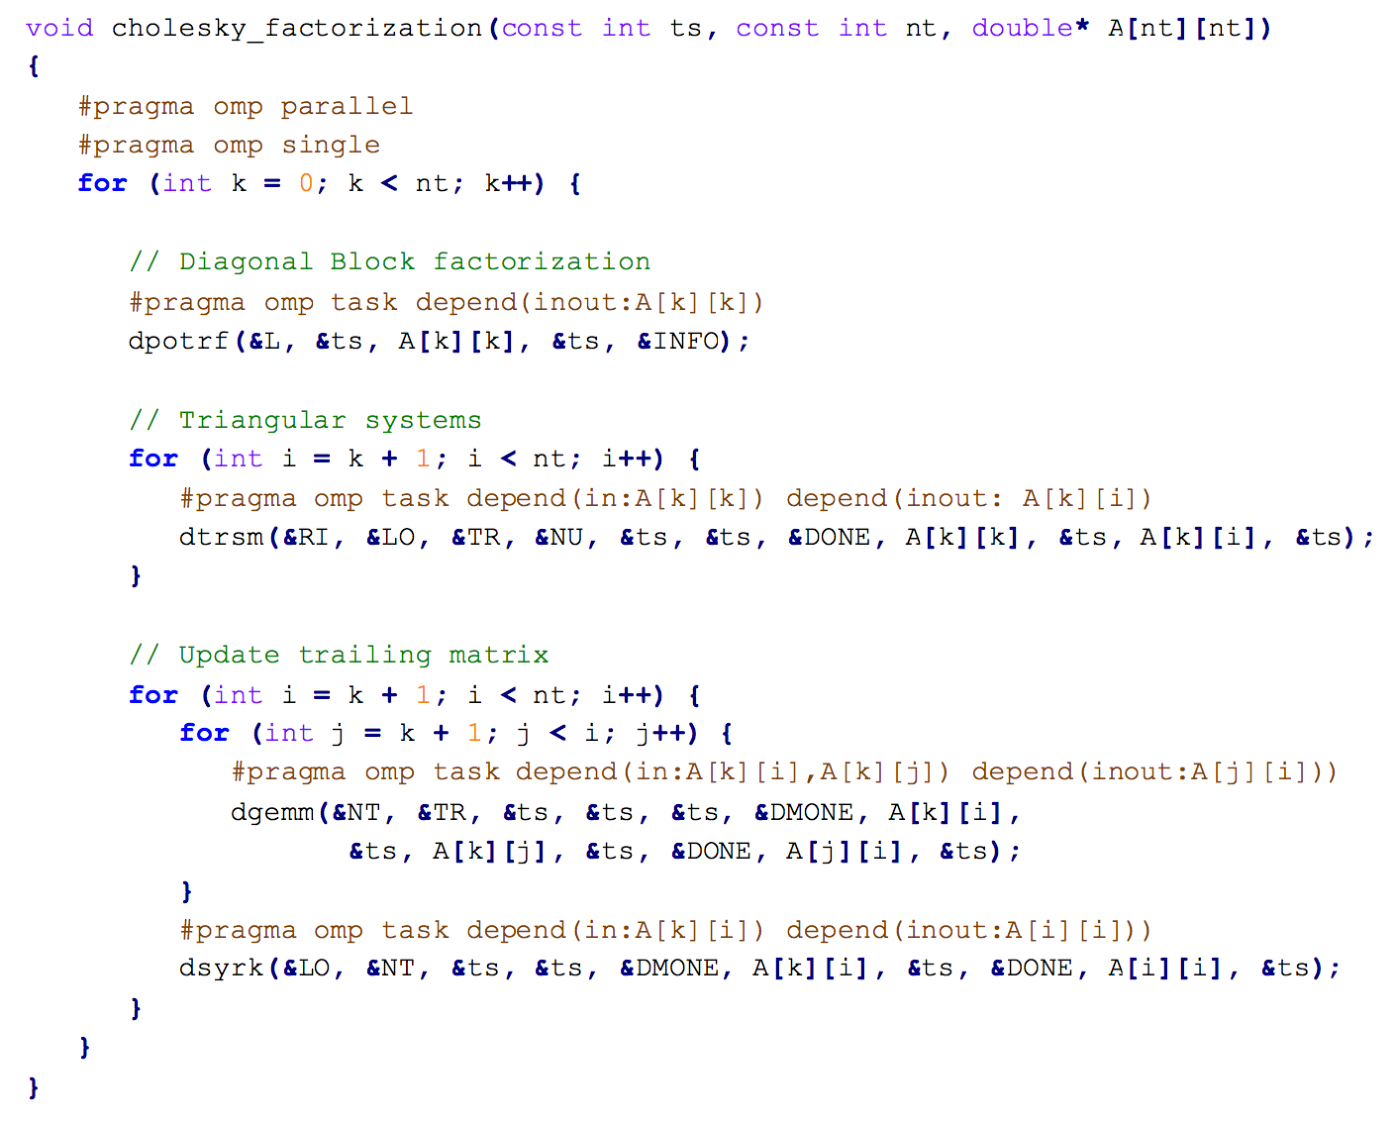
\includegraphics[width=0.75\textwidth]{images/cholesky}
%      \caption{The Mixed Use of OpenMP Tasking and Intel MKL Library for Cholesky Factorization~\cite{intertwine}}
% \label{fig:cholesky}
%\end{figure}
